\subsection{完全格序空间的子空间与积空间}

设 E 是完全格序空间，H 是 E 的一个线性子空间。E 的序结构在 H 上诱导的序结构与 H 的向量空间结构相容，但如此定义的序向量空间 H 不一定是完全格序空间。

更确切地说，可能发生 H 不是 Riesz 空间的情形（习题 2），或者 H 是 Riesz 空间但不完全格序的情形：后者例如子空间 \(\mathcal{C}(\mathbf{R})\) （它含于空间 \(\mathcal{B}(\mathbf{R})\) ）的情形（No. 3, 例 2）。

\pandocbounded{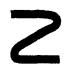
\includegraphics[keepaspectratio]{images/part001_ed0b989f.jpg}}

此外，若 H 是 Riesz 空间（不论是否完全格序），H 中两个元素在 H 中的上确界仍可能不同于它们在 E 中的上确界（习题 3 b)）。最后，还可能发生这样的情形：H 是完全格序的，H 的每个有限子集的上确界在 E 中与在 H 中相同，但存在 H 的在 H 中有上界的无限子集，它们在 E 中与在 H 中的上确界不同（习题 13 f)）。

设 \((\mathrm{E}_{\iota})_{\iota \in \mathrm{I}}\) 是任意一族序向量空间。回顾一下，在积空间 \(\mathrm{E} = \prod_{\iota \in \mathrm{I}}\mathrm{E}_{\iota}\) 中，诸因子空间的序关系的乘积序关系就是关系 \(\ll x_{\iota}\leqslant y_{\iota}\) 对一切 \(\iota \in \mathrm{I}\gg (\mathrm{S},\mathrm{III},\S 1,\mathrm{No.~4})\)。立即可验证这一关系与 E 的向量空间结构相容；赋以这一结构的 E 称为诸序空间 \(E_{\iota}\) 的积空间。

命题 3. --- 设 \((\mathbf{E}_{\iota})_{\iota\in\mathbb{I}}\) 是一族序向量空间。为使积空间 \(E=\prod_{\iota\in I}E_{\iota}\) 是 Riesz 空间（相应地，完全格序空间），必要且充分的是：每个空间 \(E_{\iota}\) 都是 Riesz 空间（相应地，完全格序空间）。

我们只限于考察完全格序空间的情形。设所有 \(E_{\iota}\) 都是完全格序的；设 A 是 E 的一个有上界的非空子集，\(a = (a_{\iota})\) 是 A 的一个上界。对每个 \(\iota \in I\) ，\(pr_{\iota}A\) 以 \(a_{\iota}\) 为上界，因而有上确界 \(b_{\iota}\) （在 \(E_{\iota}\) 中）；显然 \(b = (b_{\iota})\) 是 A 在 E 中的上确界。

反过来，设 E 是完全格序的。设 \(A_{\kappa}\) 是 \(E_{\kappa}\) 的一个有上界的子集，\(A_{\kappa}^{\prime}\) 是 E 中由那些 \(x = (x_{\iota})\) （它们满足 \(x_{\kappa} \in A_{\kappa}\) 且 \(x_{\iota} = 0\) 对 \(\iota \neq \kappa\) ）所组成的子集。立即可以看出 \(A_{\kappa}^{\prime}\) 在 E 中有上界，因而有上确界 \(b = (b_{\iota})\) ；由乘积序关系的定义，必有 \(b_{\iota} = 0\) （对 \(\iota \neq \kappa\) ），而 \(b_{\kappa}\) 是 \(A_{\kappa}\) 的上确界，证毕。

定义 3. --- 设 E 是一个序向量空间，V 与 W 是 E 的两个互补线性子空间。若典范映射 \((x,y)\mapsto x+y\) （把序向量空间 \(V\times W\) 映到序向量空间 E 上）是一个同构，则称 E 是 V 与 W 的序直和。

命题 4. --- 为使序向量空间 E 是两个互补线性子空间 V, W 的序直和，必要且充分的是：关系 \(x \in V\) 、\(y \in W\) 、\(x + y \geqslant 0\) 蕴涵 \(x \geqslant 0\) 与 \(y \geqslant 0\) 。

由于在 E 中 \(x \geqslant 0\) 与 \(y \geqslant 0\) 蕴涵 \(x + y \geqslant 0\) ，命题中的条件表明 \((x, y) \mapsto x + y\) 把由元素 \(\geqslant 0\) 组成的集（取自 \(V \times W\) ）变换为由元素 \(\geqslant 0\) 组成的集（取自 E）。

